\documentclass[11pt,letterpaper]{article}
\usepackage[utf8]{inputenc}
\usepackage[T1]{fontenc}
\usepackage[spanish,es-tabla]{babel}
\usepackage[margin=2.4cm]{geometry}
\usepackage{graphicx,booktabs,amsmath,xcolor}
\usepackage[colorlinks=true,urlcolor=teal,linkcolor=teal,citecolor=teal]{hyperref}
\hypersetup{pdftitle={Riesgo tarifario y tamaño de posición en GAPB},pdfauthor={Francisco Uriel Ledezma Chávez}}
\graphicspath{{./}{../docs/04-variance-models_files/figure-html/}}
\setlength{\parindent}{0pt}\setlength{\parskip}{0.55em}
\raggedbottom
\begin{document}
{\small\color{teal}\textbf{ESTUDIO DE CASO}\hfill Ingeniería Financiera · ITESO}\par
\rule{\linewidth}{0.5pt}\par
{\LARGE\bfseries Riesgo tarifario y tamaño de posición en GAPB}\par
{\large Evidencia diaria de una cartera de seis acciones mexicanas}\par
Francisco Uriel Ledezma Chávez \hfill 25 de noviembre de 2026

\textbf{Resumen.} ¿Cuánto cambia la lectura del riesgo de Grupo Aeroportuario del Pacífico cuando la unidad de análisis pasa de la acción a una cartera? El 5 de octubre de 2023, GAPB cayó 22.45\%. Al reproducir esa sesión en una cartera con seis posiciones iguales, la emisora explica 81.2\% de la pérdida. En la reconstrucción del episodio, la volatilidad estimada por GARCH pasó de 2.59\% a 10.08\% diario. Al corte de noviembre de 2026, el VaR histórico diario de la cartera al 99\% superó al normal en 7,596 pesos, pero la diferencia se redujo a 790 pesos al igualar las ventanas. En 222 sesiones posteriores a sus respectivas fechas de pronóstico, el histórico registró una excepción y el normal tres. La asignación de menor VaR normal conservó un peso de 6.05\% en GAPB. El caso distingue tres decisiones con exigencias de evidencia distintas: cuándo revisar una posición, cuánto reservar para pérdidas y cuánto capital asignar a la emisora.

\textit{Palabras clave:} regulación tarifaria, volatilidad condicional, valor en riesgo, concentración.
\section{El episodio que motiva la pregunta}
GAP opera aeropuertos bajo concesión. En México, una tarifa máxima condiciona el ingreso que puede obtener por determinados servicios aeronáuticos. Una modificación a sus bases altera las expectativas de cobro incluso si el tráfico de pasajeros permanece constante. Para dimensionar esa exposición, en 2025 los servicios aeronáuticos aportaron aproximadamente 70\% del ingreso operativo consolidado, excluida la construcción bajo IFRIC~12 \cite{proyecto}. Esta mezcla posterior al episodio describe el negocio y comprende operaciones fuera de México.

El 4 de octubre de 2023, GAP comunicó que la autoridad había modificado las bases de regulación tarifaria \cite{gap}. En la sesión siguiente, 100,000 pesos expuestos a GAPB habrían perdido 22,451 pesos. Las otras cinco posiciones de igual monto habrían perdido juntas 5,195 pesos, para una pérdida total de 27,645 pesos al redondear la suma de los importes originales. La coincidencia temporal y el mecanismo de ingresos justifican estudiar esa jornada. Aislar la fracción del movimiento causada por el anuncio requeriría un contrafactual.

\newpage
\section{La velocidad y el costo de una alerta}
Se emplearon rendimientos logarítmicos diarios de cierres ajustados de GAPB. Dentro de las 1,445 sesiones de enero de 2021 a septiembre de 2026, el primer 70\% sirvió para estimar parámetros y el 30\% restante, para evaluar y seleccionar especificaciones. Se compararon un promedio móvil de 40 sesiones, el promedio exponencial (EWMA), su variante basada en datos (DDEWMA) y un GARCH(1,1) con media autorregresiva. Este último actualiza la varianza por medio de la innovación al cuadrado y de la varianza anterior \cite{bollerslev}. Por ello, un movimiento extremo en cualquier dirección puede elevar su siguiente pronóstico.

\begin{center}
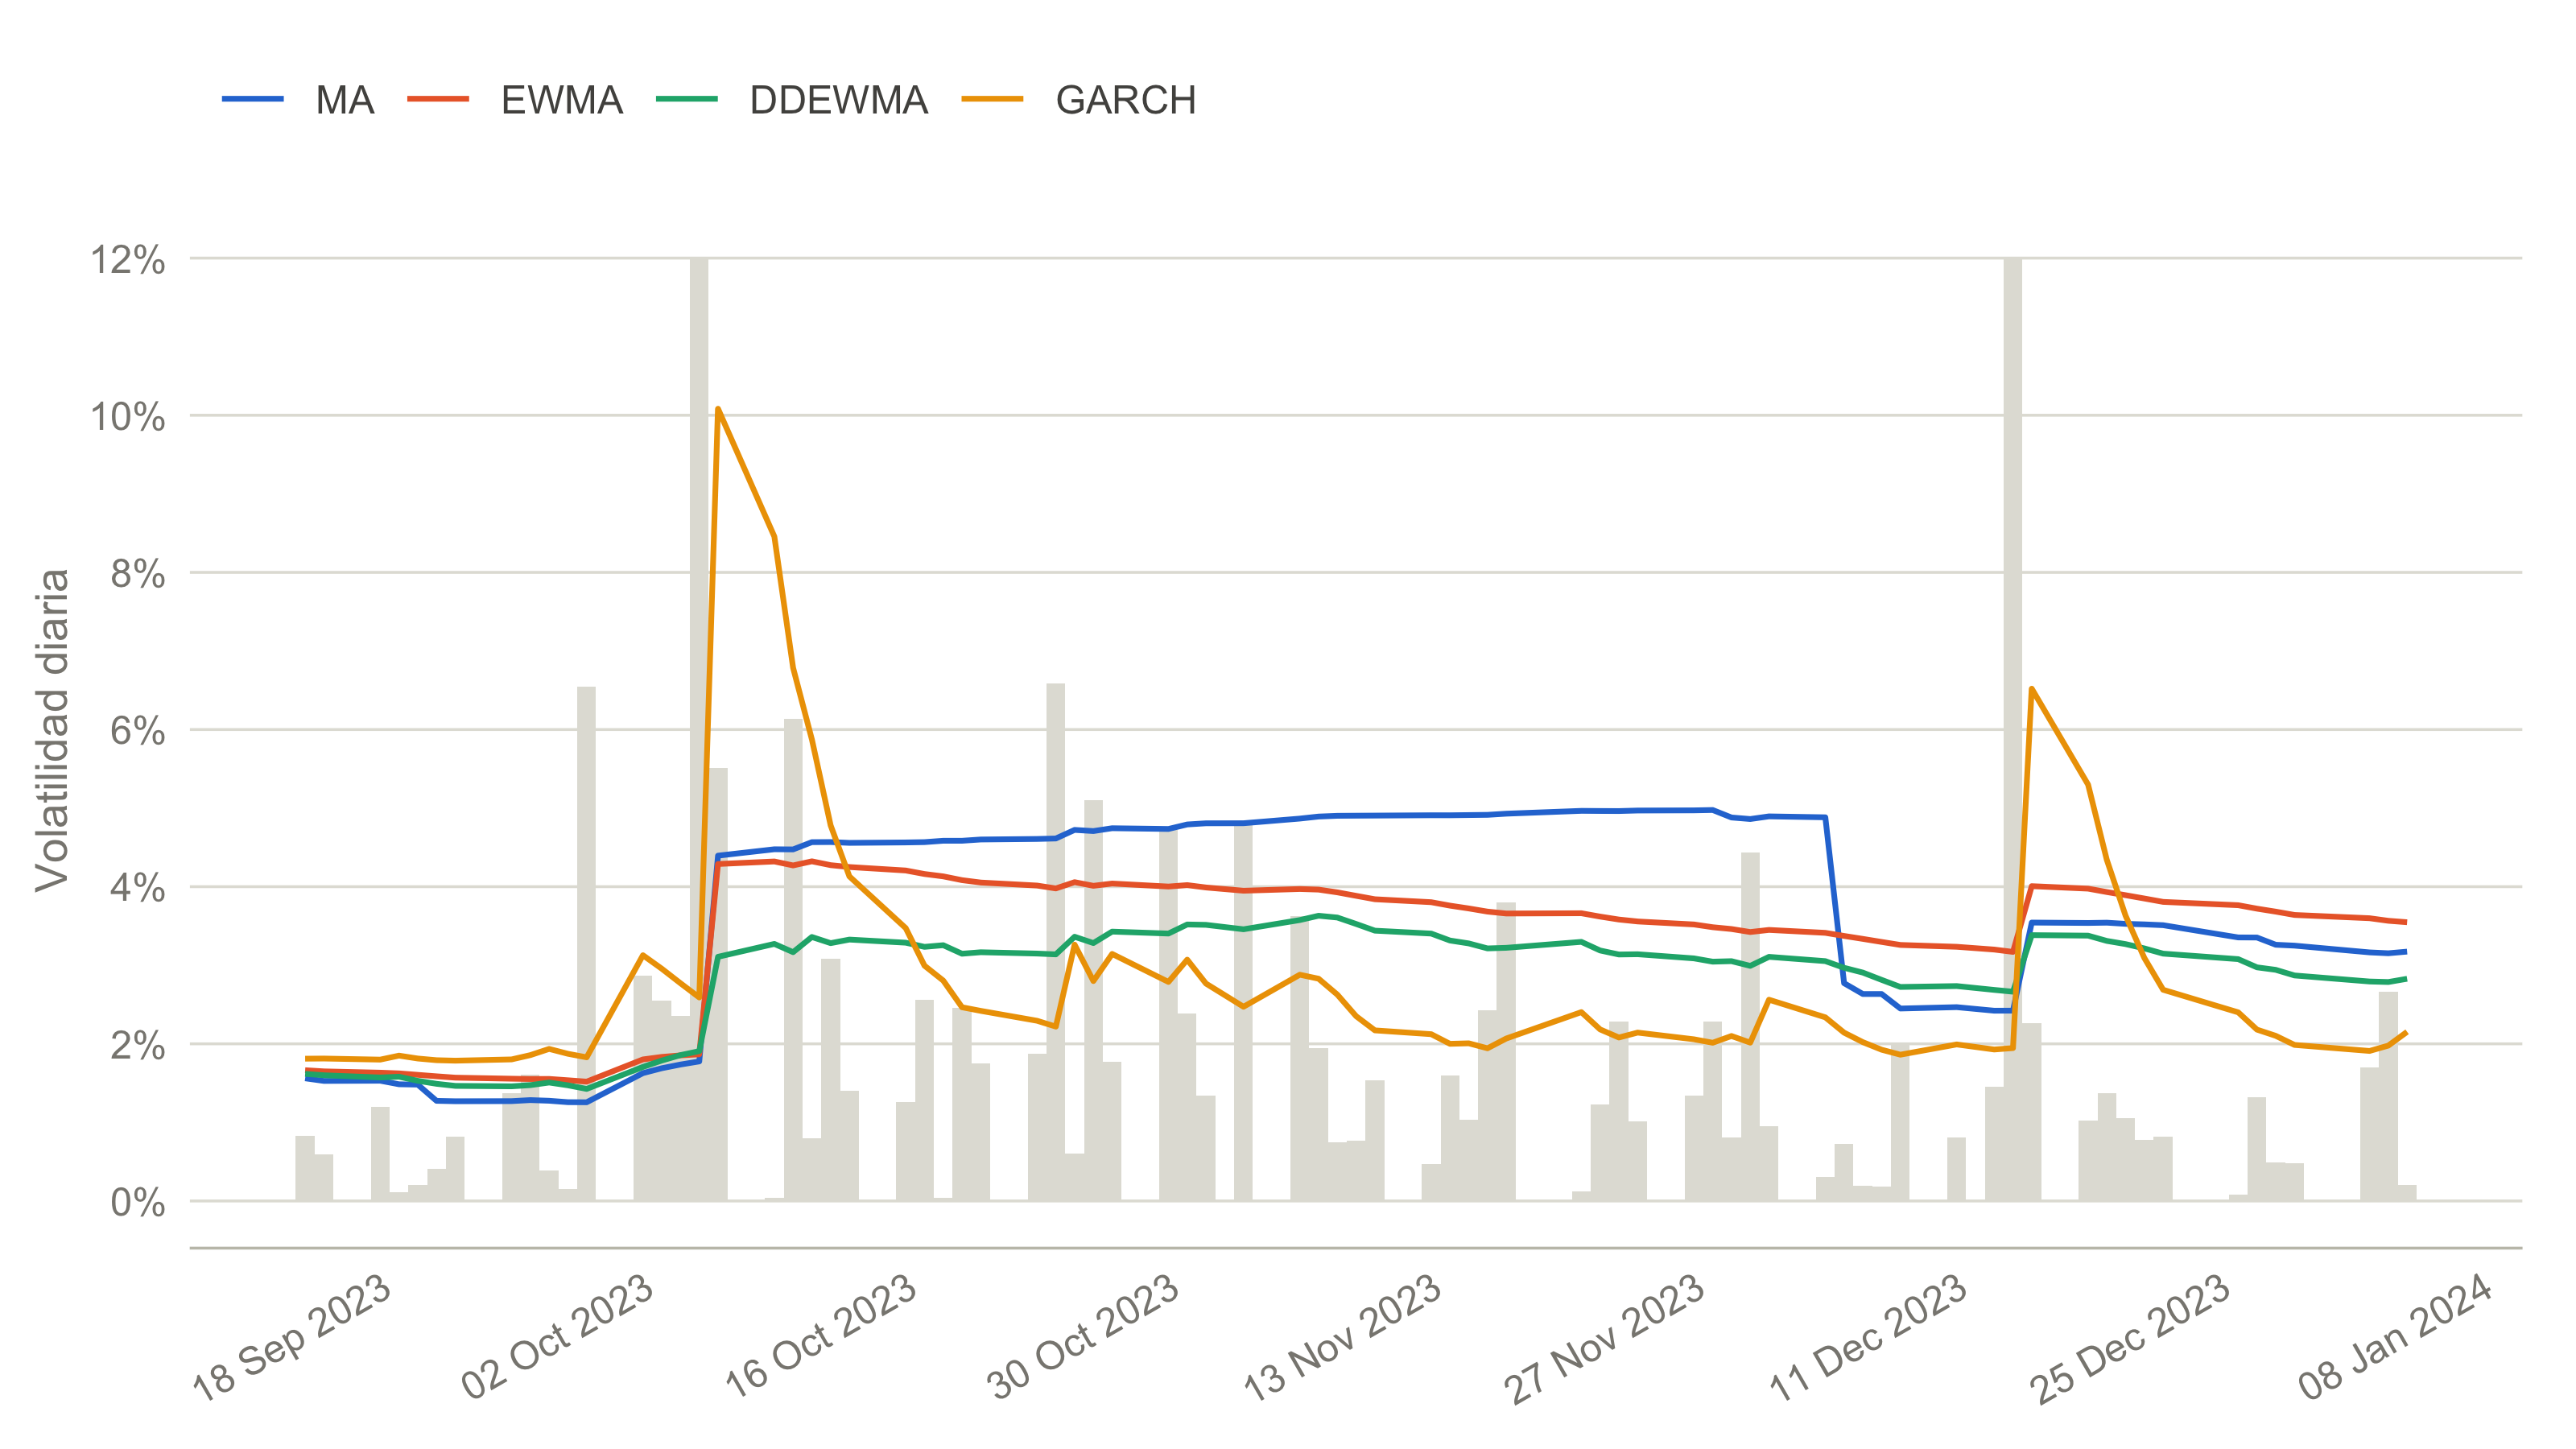
\includegraphics[width=0.94\linewidth]{fig-shock-1.png}\\
{\small\textbf{Figura 1.} Respuesta de los cuatro modelos en torno al choque de octubre de 2023. El rendimiento logarítmico absoluto se muestra hasta 12\% para facilitar la comparación. Fuente: Parte 4 del proyecto \cite{proyecto}.}
\end{center}

La caída simple de 22.45\% equivale a una caída logarítmica de 25.43\%. Al incorporar esa observación, la volatilidad diaria del GARCH pasó de 2.59\% a 10.08\%, un múltiplo de 3.89 frente a 2.30 para el EWMA. En cuatro sesiones se había disipado al menos la mitad del repunte. Esta reconstrucción usa parámetros estimados con datos hasta enero de 2025, de modo que permite comparar reacciones a un mismo choque sin atribuirle al gestor de 2023 información posterior.

La rapidez resultó útil sobre todo en los seis meses más volátiles de la evaluación. La razón entre varianza pronosticada y realizada fue de 0.94 para GARCH y 0.75 para EWMA; en los demás meses pasó a 1.54 y 1.21, respectivamente. El GARCH habría dado una señal más intensa para revisar límites tras el salto, con el costo de sobrestimar más la varianza en periodos tranquilos. La clasificación de meses se conoce una vez observados sus rendimientos.

\newpage
\section{Magnitud de la pérdida y cobertura del límite}
Al cierre del 23 de noviembre de 2026 se valuaron posiciones de 100,000 pesos en ALSEA, Banco del Bajío, GAPB, Grupo México, Orbia y Walmart de México. Para simular la pérdida de la cartera actual se aplicaron los rendimientos simples conjuntos de cada fecha a sus pesos iniciales. La historia aporta 2,376 rendimientos diarios comunes desde junio de 2017. El método histórico toma el percentil 99 de las pérdidas. Bajo normalidad y media cero, el límite a un día es
\[
  \mathrm{VaR}_{0.99}= S_0\,\Phi^{-1}(0.99)\sqrt{w^\top\Sigma w},
\]
donde $S_0=600{,}000$ pesos y $\Sigma$ es la covarianza diaria estimada con las 128 sesiones comunes de los últimos seis meses.

\begin{center}
\textbf{Tabla 1.} Sensibilidad del VaR diario al 99\% a la ventana\\[5pt]
\begin{tabular}{lrr}\toprule
Método & Sesiones & VaR (MXN)\\ \midrule
Histórico, muestra común completa & 2,376 & 19,652\\
Histórico, ventana reciente & 128 & 12,846\\
Normal, ventana reciente & 128 & 12,056\\ \bottomrule
\end{tabular}
\end{center}
La diferencia entre los extremos de la tabla es 7,596 pesos. Al restringir ambos métodos a las mismas fechas quedan 790 pesos de diferencia. La elección de la muestra influye materialmente en el capital sugerido. El percentil reciente depende de apenas dos o tres observaciones de cola, por lo que su cercanía al normal ofrece evidencia limitada acerca de la forma de la distribución. En la historia completa, la pérdida promedio del peor 1\% de escenarios, o \textit{Expected Shortfall}, llegó a 30,606 pesos.

\begin{center}
\textbf{Tabla 2.} Excepciones en 222 pronósticos diarios durante 2026\\[5pt]
\begin{tabular}{lrrr}\toprule
Confianza & Esperadas & Histórico & Normal\\ \midrule
95\% & 11.10 & 8 & 7\\
97.5\% & 5.55 & 5 & 6\\
99\% & 2.22 & 1 & 3\\ \bottomrule
\end{tabular}
\end{center}
Para cada sesión se reconstruyó el límite con los datos disponibles al cierre anterior. El histórico amplió su muestra y el normal desplazó su ventana de seis meses. Al 99\%, los valores $p$ de cobertura incondicional de Kupiec \cite{kupiec} fueron 0.36 y 0.62. A un nivel de significancia de 5\%, ambos conteos son compatibles con la tasa nominal. Con solo 2.22 excepciones esperadas, esta prueba distingue con dificultad entre métodos y deja abierta la posibilidad de que las pérdidas extremas se agrupen.

\newpage
\section{Decisión de cartera y límites del resultado}
Para el mismo valor de cartera y con media cero, minimizar el VaR normal equivale a minimizar $w^\top\Sigma w$. Se exigió invertir todo el capital, con posiciones largas y un máximo de 40\% por emisora. El cambio de composición redujo en 801 pesos el umbral normal diario y dejó 36,297 pesos en GAPB. Los dos portafolios también se revaluaron con idénticos movimientos históricos.

\begin{center}
\textbf{Tabla 3.} Dos asignaciones de 600,000 pesos al mismo corte\\[5pt]
\begin{tabular}{lrr}\toprule
Medida & Equiponderada & Mínimo VaR normal\\ \midrule
Peso de GAPB & 16.67\% & 6.05\%\\
VaR normal diario al 99\% (MXN) & 12,056 & 11,255\\
VaR histórico diario al 99\% (MXN) & 19,652 & 18,113\\
Número efectivo de emisoras & 6.00 & 4.74\\ \bottomrule
\end{tabular}
\end{center}
El capital se concentró en Walmart y Banco del Bajío, que juntos recibieron 56.35\%. El número efectivo de emisoras, $1/\sum_i w_i^2$, cayó aunque también descendió la varianza estimada. La reducción se explica por la combinación completa de pesos y covarianzas. El backtesting de la tabla 2 corresponde a la cartera equiponderada, por lo que no demuestra que la asignación optimizada vaya a ahorrar 801 pesos en una sesión futura.

\textbf{Conclusión.} Para esta cartera conservaría GAPB con un peso cercano al 6\%. El episodio regulatorio muestra por qué una sexta parte del capital puede dominar la pérdida de una jornada; la covarianza con las demás posiciones aporta el criterio cuantitativo para dimensionarla. Revisaría la decisión si cambian las bases tarifarias, las covarianzas o el objetivo del inversionista. El estudio estima exposición a pérdidas y deja sin resolver la compensación que ofrecería la emisora en rendimiento esperado.

{\small\textbf{Procedencia y reproducción.} Manuscrito individual basado en el proyecto académico de equipo \cite{proyecto}. Los reportes 1, 2, 4 y 5 documentan el negocio, la cronología y las estimaciones. El conjunto de precios congelado de la Parte 5, las funciones en R y los reportes ejecutables están en la versión citada del repositorio.}
{\small
\begin{thebibliography}{9}\setlength{\itemsep}{1pt}
\bibitem{bollerslev} Bollerslev, T. (1986). Generalized autoregressive conditional heteroskedasticity. \textit{Journal of Econometrics}, 31, 307--327. \href{https://doi.org/10.1016/0304-4076(86)90063-1}{DOI}.
\bibitem{kupiec} Kupiec, P. (1995). Techniques for verifying the accuracy of risk measurement models. \textit{The Journal of Derivatives}, 3(2), 73--84. \href{https://doi.org/10.3905/jod.1995.407942}{DOI}.
\bibitem{gap} Grupo Aeroportuario del Pacífico (2023). \href{https://www.globenewswire.com/news-release/2023/10/05/2755031/0/en/Grupo-Aeroportuario-del-Pacifico-Announces-Government-Action-to-Change-Tariff-Base-Regulation.html}{Announces Government Action to Change Tariff Base Regulation}. Comunicado del 4 de octubre.
\bibitem{proyecto} Proyecto GAPB, ITESO (2026). \href{https://github.com/Urielledezma/GAPB-Risk-Analysis/tree/adda9699c88f6b211b9287ee4735621c97d1f1ed}{Análisis del riesgo de mercado de GAPB. Datos, código y cinco reportes}.
\end{thebibliography}}
\end{document}
